\documentclass[openright, a4paper]{article}
\usepackage{graphicx}
\usepackage{kotex}
\usepackage{minted}
\usepackage{setspace}
\usepackage{underscore}
\usepackage{caption}
\usepackage[margin=3cm]{geometry}
\newcommand{\code}[1]{\texttt{#1}}
\captionsetup{labelformat=empty,labelsep=none}

\title{2024학년도 컴퓨터구조 Lab Assignment \#2\\
        Single Cycle CPU}

\author{김도영, 선민수}
\date{2024년 3월 25일}

\onehalfspacing
\begin{document}

\maketitle

\section{Introduction}
이 과제에서는 Verilog를 이용하여 Single Cycle CPU를 구현하는 것을 목적으로 한다.


\section{Design}
본 과제에서 구현한 Single Cycle CPU는 수업 시간에 배운 Data Path를 기준으로 구현하였으며, 추가적인 LUI, AUIPC Instruction을 위한 Data Path 또한 구현하였다.

{
    \begin{figure}[!h]
        \centering
        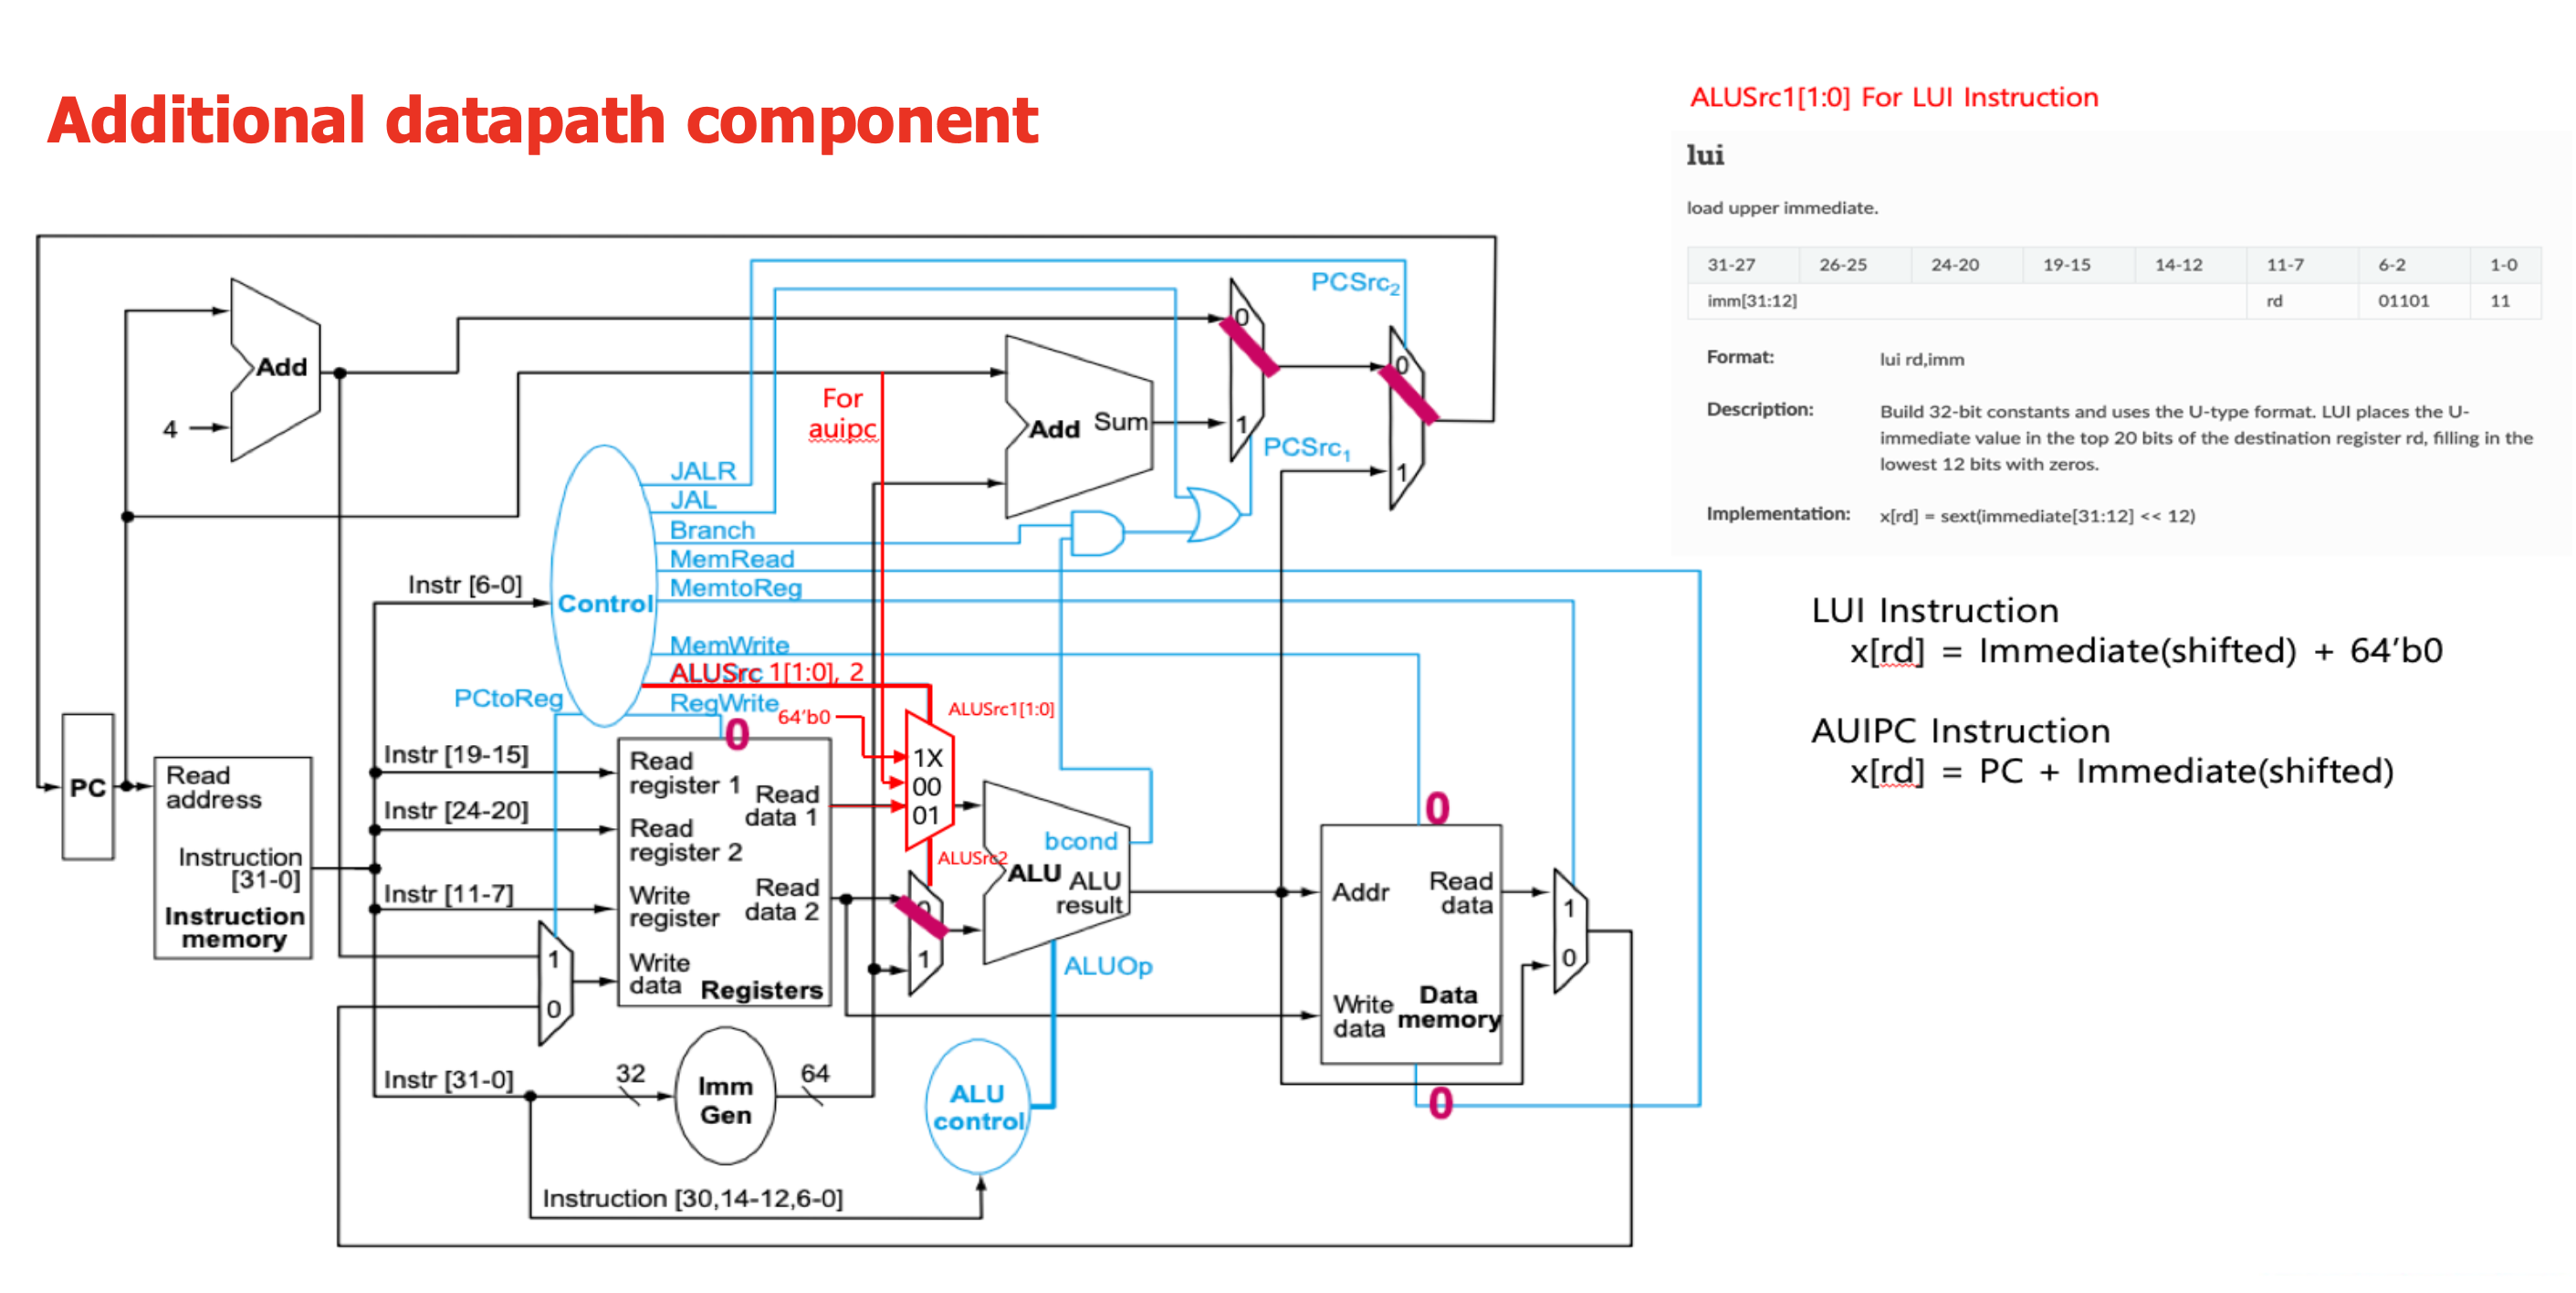
\includegraphics[width=\textwidth]{Design.png}
        \label{fig:design}
        \caption{Design of Single-Cycle CPU}
    \end{figure}
}

Single Cycle CPU를 구성하는 세부 모듈들과 각각의 역할은 아래와 같다.

\hfill

\begin{itemize}
    \item ALU Control Unit: Instruction에서 ALU가 필요한 OPCode, Funct3, Funct7을 추출하여 ALU에 alu_op로 전달한다.
    \item ALU: alu_op을 이용하여 현재 필요한 연산을 결정하고, 이에 대한 연산을 입력을 이용해 결과를 도출한다. BRANCH Instruction의 경우 bcond 출력을 이용해 BRANCH taken/not-taken을 출력한다.
    \item Control Unit: 주어진 Instruction을 이용하여 종류를 판단하고 필요한 Control Value를 출력한다.
    \item Data Memory: 프로그램에 필요한 데이터가 저장되는 메인 메모리로, 주어진 주소에 대한 데이터를 출력하거나, mem_write 신호에 따라 메모리에 데이터를 넣기도 한다. 이번 과제에서는 주어진 지시에 따라 Synchronous Data Write, Asynchronous Data Read의 메모리를 구현한다.
    \item Immediate Generator: Immediate가 사용되는 Instruction의 종류에 따라서 Immediate를 추출하여 imm_gen_out으로 출력한다.
    \item Instruction Memory: Instruction을 CPU에 불러오는 Memory이다. Data Memory와 달리 Instruction만이 저장되어 있으며, 새로운 데이터가 작성되는 일은 없다. Data Memory와 같이 주어진 주소에 대한 Instruction을 출력한다. 이번 과제에서는 주어진 지시에 따라 Asynchronous Instruction Read의 메모리를 구현한다.
    \item Next PC: Program Counter의 다음 값을 결정하는 모듈로, 위의 디자인 그림에서는 따로 구분되어 있지 않지만, Program Counter의 다음 값을 결정하는 Data Path를 모듈화한 모듈이다. JAL, JALR, BRANCH Instruction인지 판단하여 ALU의 결과값과 Immediate 값을 이용해 다음 Program Counter의 값을 결정한다.
    \item Program Counter: 주어진 next_pc 값으로 Program Counter를 변화시킨다.
    \item Register File: 주어진 Register 번호에 대한 Register의 데이터를 출력한다. write_enable 신호에 의해 대상 register에 값을 쓰기도 한다.
    \item CPU: 위의 모듈들을 관리하는 top module로, 전체 모듈들을 연결하며, 과제의 조건에 따라 instruction이 ecall인 경우 10번 레지스터의 값이 10이 될 때, 종료 신호를 출력한다.
\end{itemize}

\hfill

Single Cycle CPU는 아래와 같은 단게를 통해 Instruction을 수행하게 된다.

\begin{itemize}
    \item Instruction Fetch Stage: 이전 Instruction에 의해 결정된 next_pc를 이용하여 current_pc를 업데이트한 후 이를 통해서 Instruction Memory의 Instruction을 패치한다. Program Counter와 Next Program Counter Logic이 주축이 되어 해당 스테이지를 처리한다.
    \item Instruction Decode Stage: Instruction Fetch를 통해 얻은 Instruction을 필요한 데이터로 가공 및 추출한다. 동시에 Register File에서 필요한 레지스터를 읽어온다. Control Unit, ALU Control Unit, Register File을 주축으로 하여 해당 스테이지를 처리한다.
    \item Execution Stage: 주어진 Instruction과 추출된 데이터를 기반으로 연산을 진행한다. 동시에 BRANCH Instruction의 경우에는 bcond 신호를 결정한다. ALU가 해당 스테이지를 처리한다.
    \item Access Memory Stage: ALU에서 추출된 결과를 통해서 필요한 메모리의 주소를 계산한 후, Data Memory에서 해당 주소의 데이터를 읽는다. Instruction에 따라서 Write가 필요한 경우에는 mem_write를 통해 Memory에 데이터를 쓰도록 한다. Memory가 해당 스테이지를 처리한다.
    \item Write Back Stage: 연산 결과 혹은 메모리에서 읽은 데이터를 레지스터에 다시 쓰는 스테이지이다. Register File의 rd, din을 이용하여 write_enable에 따라 레지스터에 데이터를 쓰게 된다. Register File이 해당 스테이지를 관리한다.
\end{itemize}

\section{Implementation}

\subsection{Program Counter}

\begin{figure}[h]
    \begin{minted}[fontsize=\footnotesize]{Verilog}
always @(posedge clk) begin
    if (reset) begin
        current_pc <= 0;
    end else begin
        current_pc <= next_pc;
    end
end
    \end{minted}
    \caption{pc.v}
\end{figure}

Program Counter는 주어진 clk에 따라서 current_pc를 next_pc로 업데이트하는 Synchronous 모듈로 구현되었다.

\subsection{Next Program Counter Logic}

\begin{figure}[h]
    \begin{minted}[fontsize=\footnotesize]{Verilog}
always @(*) begin
    if(is_jalr) begin
        next_pc = alu_result;
    end else begin
        if(branch && alu_bcond || is_jal)
            next_pc = current_pc + immediate;
        else
            next_pc = current_pc + 4;
    end
end
    \end{minted}
    \caption{next_pc_logic.v}
\end{figure}

Next Program Counter Logic은 주어진 is_jalr, branch, alu_bcond, is_jal 신호에 따라서 다음 Program Counter 값을 Asynchronous하게 산출하는 모듈이다.

\subsection{Control Unit}

\begin{figure}[!h]
    \begin{minted}[fontsize=\footnotesize]{Verilog}
always @(*) begin
    is_jal = (opcode == `JAL);
    is_jalr = (opcode == `JALR);
    branch = (opcode == `BRANCH);
    mem_read = (opcode == `LOAD);
    mem_to_reg = (opcode == `LOAD);
    mem_write = (opcode == `STORE);
    alu_src_1[1] = (opcode == `LUI);
    alu_src_1[0] = (opcode == `AUIPC);
    alu_src_2 = ((opcode != `ARITHMETIC) && (opcode != `BRANCH));
    write_enable = ((opcode != `STORE) && (opcode != `BRANCH));
    pc_to_reg = (opcode == `JALR || opcode == `JAL);
    is_ecall = (opcode == `ECALL);
end
    \end{minted}
    \caption{control_unit.v}
\end{figure}

Control Unit은 주어진 instruction에서 opcode에 따라 필요한 Control Value를 계산하여 산출하는 Asynchronous 모듈이다.

\subsection{ALU Control Unit}

\begin{figure}[!h]
    \begin{minted}[fontsize=\footnotesize]{Verilog}
always @(*) begin
    alu_op = {funct7, funct3, opcode};
end
    \end{minted}
    \caption{alu_ctrl_unit.v}
\end{figure}

ALU Control Unit은 주어진 funct3, funct7, opcode를 합쳐 alu_op 신호를 통해 ALU에 전달하는 Asynchronous 모듈이다.

\subsection{Immediate Generator}

\begin{figure}[!h]
    \begin{minted}[fontsize=\footnotesize]{Verilog}
always @(*) begin
    case(opcode)
    `ARITHMETIC_IMM: imm_gen_out = {{20{inst[31]}}, inst[31:20]};
    `LOAD          : imm_gen_out = {{20{inst[31]}}, inst[31:20]};
    `STORE         : imm_gen_out = {{20{inst[31]}}, inst[31:25], inst[11:7]};
    `BRANCH        : imm_gen_out = {{19{inst[31]}}, inst[31], inst[7], inst[30:25], inst[11:8], 1'b0};
    `JAL           : imm_gen_out = {{11{inst[31]}}, inst[31], inst[19:12], inst[20], inst[30:21], 1'b0};
    `LUI           : imm_gen_out = {inst[31:12], 12'b0};
    `AUIPC         : imm_gen_out = {inst[31:12], 12'b0};
    default        : imm_gen_out = {32{1'b0}};
    endcase
end
    \end{minted}
    \caption{imm_gen.v}
\end{figure}

Immediate Generator는 주어진 instruction의 opcode에 따라서 immediate value를 추출하는 Asynchronous 모듈이다. Immediate value가 필요하지 않을 경우 32'b0으로 출력한다.

\subsection{Register File}

\begin{figure}[h]
    \begin{minted}[fontsize=\footnotesize]{Verilog}
// Asynchronously read register file
always @(*) begin
    rs1_dout = (rs1 == 5'b0) ? 32'b0 : rf[rs1];
    rs2_dout = (rs2 == 5'b0) ? 32'b0 : rf[rs2];
end

// Synchronously write data to the register file
always @(posedge clk) begin
    if (write_enable)
        rf[rd] <= rd_din;
end
    \end{minted}
    \caption{register_file.v}
\end{figure}

Register File은 주어진 rs1, rs2에 따라 해당 레지스터의 값을 Asynchronous하게 출력하고, clk에 맞추어 rd에 해당하는 레지스터에 din 값을 Synchronous하게 쓴다. x0의 경우에는 rs1과 rs2 신호를 읽는 과정에서 해당 경우를 검출하고, 0을 출력하도록 구현하였다.

\newpage

\subsection{ALU}
\begin{figure}[!h]
    \begin{minted}[fontsize=\footnotesize]{Verilog}
    always @(*) begin
        case(opcode)
        `ARITHMETIC: begin
            alu_bcond = 1'b0;
            if(funct7 != `FUNCT7_SUB) begin
                case(funct3)
                `FUNCT3_ADD: alu_result = alu_in_1 + alu_in_2;
                `FUNCT3_SLL: alu_result = alu_in_1 << alu_in_2;
                `FUNCT3_XOR: alu_result = alu_in_1 ^ alu_in_2;
                `FUNCT3_SRL: alu_result = alu_in_1 >> alu_in_2;
                `FUNCT3_OR : alu_result = alu_in_1 | alu_in_2;
                `FUNCT3_AND: alu_result = alu_in_1 & alu_in_2;
                default    : alu_result = 32'b0;
                endcase
            end else begin
                alu_result = alu_in_1 - alu_in_2;
            end
        end

        `ARITHMETIC_IMM: begin
            alu_bcond = 1'b0;
            case(funct3)
            `FUNCT3_ADD: alu_result = alu_in_1 + alu_in_2;
            `FUNCT3_SLL: alu_result = alu_in_1 << alu_in_2;
            `FUNCT3_XOR: alu_result = alu_in_1 ^ alu_in_2;
            `FUNCT3_OR : alu_result = alu_in_1 | alu_in_2;
            `FUNCT3_AND: alu_result = alu_in_1 & alu_in_2;
            `FUNCT3_SRL: alu_result = alu_in_1 >> alu_in_2;
            default    : alu_result = 32'b0;
            endcase
        end
    \end{minted}
    \caption{alu.v}
\end{figure}
\begin{figure}[!h]
    \begin{minted}[fontsize=\footnotesize]{Verilog}
        `LOAD: begin
            alu_bcond = 1'b0;
            alu_result = alu_in_1 + alu_in_2;
        end

        `JALR: begin
            alu_bcond = 1'b0;
            alu_result = alu_in_1 + alu_in_2;
        end

        `STORE: begin
            alu_bcond = 1'b0;
            alu_result = alu_in_1 + alu_in_2;
        end

        `BRANCH: begin
            alu_result = 32'b0;
            case(funct3)
            `FUNCT3_BEQ: alu_bcond = (alu_in_1 == alu_in_2);
            `FUNCT3_BNE: alu_bcond = (alu_in_1 != alu_in_2);
            `FUNCT3_BLT: alu_bcond = (alu_in_1 < alu_in_2);
            `FUNCT3_BGE: alu_bcond = (alu_in_1 >= alu_in_2);
            default    : alu_bcond = 1'b0; 
            endcase
        end
    \end{minted}
    \caption{alu.v}
\end{figure}
\begin{figure}[!h]
    \begin{minted}[fontsize=\footnotesize]{Verilog}
        `JAL: begin
            alu_result = 32'b0;
            alu_bcond = 1'b0;
        end

        `LUI: begin
            alu_result = alu_in_1 + alu_in_2;
            alu_bcond = 1'b0;
        end

        `AUIPC: begin
            alu_result = alu_in_1 + alu_in_2;
            alu_bcond = 1'b0;
        end

        default: begin
            alu_result = 32'b0;
            alu_bcond = 1'b0;
        end
        endcase
    end
    \end{minted}
    \caption{alu.v}
\end{figure}

ALU는 주어진 opcode, funct3, funct7과 alu_in_1, alu_in_2에 따라 연산 결과값을 계산하는 Asynchronous 모듈로 구현하였다. 주어진 instruction 이외에는 alu_result와 alu_bcond를 0으로 처리하였다.

\subsection{Instruction/Data Memory}

\begin{figure}[!h]
    \begin{minted}[fontsize=\footnotesize]{Verilog}
    // Asynchronously read instruction from the memory 
    // (use imem_addr to access memory)
    always @(*) begin
        dout = mem[imem_addr];
    end
    \end{minted}
    \caption{instruction_memory.v}
\end{figure}

\hfill \break
\begin{figure}[!h]
    \begin{minted}[fontsize=\footnotesize]{Verilog}
    // Asynchrnously read data from the memory
    // Synchronously write data to the memory
    // (use dmem_addr to access memory)
    always @(*) begin
        if(mem_read)
            dout = mem[dmem_addr];
        else
            dout = 32'b0;
    end
    always @(posedge clk) begin
        if(mem_write) begin
            mem[dmem_addr] <= din;
        end
    end
    \end{minted}
    \caption{data_memory.v}
\end{figure}

Instruction Memory와 Data Memory 모두 Memory의 기능을 하므로, 비슷한 구현을 가진다. Data Read의 경우에는 두 모듈 모두 동일하게 Asynchronous한 구현을 가지며, Data Write이 가능한 Data Memory의 경우 mem_write 신호에 따라서 din의 값을 address 위치의 메모리에 저장하는 Synchronous한 로직을 구현했다. Data Read의 경우에는 Asynchronous하지만, Control Value인 mem_read 신호가 유효한 경우에 대해서만 값이 출력되도록 구현되었다.

\subsection{CPU}

\begin{figure}[h]
    \begin{minted}[fontsize=\footnotesize]{Verilog}
always @(*) begin
if(pc_to_reg)
  rd_din = current_pc + 4;
else begin
  if(mem_to_reg)
    rd_din = data;
  else
    rd_din = alu_result;
end
end

always @(*) begin
if(alu_src_2)
  alu_in_2 = immediate;
else
  alu_in_2 = rs2_dout;
end

always @(*) begin
if(alu_src_1[1])
  alu_in_1 = 32'b0;
else if(alu_src_1[0])
  alu_in_1 = current_pc;
else
  alu_in_1 = rs1_dout;
end

always @(*) begin
if(is_ecall)
  rs1 = 5'b10001;
else
  rs1 = inst[19:15];
end

always @(*) begin
if(is_ecall && (rs1_dout == 10))
  is_halted = 1;
else
  is_halted = 0;
end

/* Omit Module Declarations ... */
    \end{minted}
    \caption{cpu.v}
\end{figure}

CPU 모듈은 위의 다른 모듈들을 이어주는 top module의 역할을 하도록 구현하였다. Design에서 제시하였던 Data Path에서의 멀티플렉서 등의 세부적인 Control Value 결정을 할 수 있도록 와이어링하였다.

과제의 요구 조건에 따라서 주어진 instruction이 ECALL이고, x17 레지스터의 값이 10인 경우에 is_halted 신호를 이용해 프로그램을 종료하도록 구현하였다. 모듈화의 장점을 최대한 이용하기 위해, is_ecall을 통해서 ECALL Instruction을 검출한 이후, ECALL인 경우 rs1 값을 instruction의 값과는 상관없이 x17을 가르키도록 한 후, 추후 rs1_dout의 값에서 10을 확인하여 종료 조건을 판단한다. 이외에는 제시된대로 NOP와 같이 아무것도 수행하지 않도록 구현하였다.

\section{Discussion}
이번 과제에서 구현한 Single Cycle CPU의 세부 모듈들과 각각의 모듈의 Clock Synchronous/Asynchronous 여부는 아래와 같다.

\begin{itemize}
    \item ALU Control Unit: Asynchronous
    \item ALU: Asynchronous
    \item Control Unit: Asynchronous
    \item Data Memory(Read Data): Asynchronous
    \item Data Memory(Write Data, Initializing, Reset): Synchronous
    \item Immediate Generator: Asynchronous
    \item Instruction Memory(Read Instruction): Asynchronous
    \item Instruction Memory(Initializing, Reset): Synchronous
    \item Next PC: Asynchronous
    \item Program Counter: Synchronous
    \item Register File(Register Read): Asynchronous
    \item Register File(Register Write, Initializing, Reset): Synchronous
\end{itemize}

추가로 구현한 LUI, AUIPC Instruction은 Design에서 언급한 전체 Data Path에서의 ALUSrc_1을 통해서 제어되도록 구현하였다. 2bit로 이루어진 ALUSrc_1이 1x이라면 LUI Instruction을 위해서 ALU의 첫 피연산자에 0을 입력하도록 하고, 00인 경우에는 AUIPC를 위하여 Program Counter의 값을 입력하도록, 01의 경우 일반적인 ALU의 역할을 수행하도록 두 개의 입력을 인가한다.


\section{Conclusion}
이번 과제에서는 모든 Instruction이 1 Cycle에 완료되는 Single Cycle CPU를 구현하였다. Instruction을 기반으로 CPU의 동작을 제어할 수 있는 다양한 Control Flag을 생성하여 CPU의 Data Path를 조정할 수 있도록 하여 1 Cycle 내에 Instruction을 수행할 수 있도록 설계하였다.

이번 Single Cycle CPU를 구현하면서, 1 Cycle을 온전히 1개의 Instruction을 수행하는 데 사용할 수 있지만, 1 Cycle의 시간 동안 다른 세부 모듈들이 낭비되고 있음을 알 수 있었고, 이를 개선한 Multi-Cycle CPU의 필요성을 느낄 수 있었다.

\end{document}